\documentclass{lehramt-informatik-haupt}
\liLadePakete{mathe,syntaxbaum,automaten}
\usepackage{tikz}
\usetikzlibrary{shapes.geometric,calc}
\begin{document}

%%%%%%%%%%%%%%%%%%%%%%%%%%%%%%%%%%%%%%%%%%%%%%%%%%%%%%%%%%%%%%%%%%%%%%%%
% Theorie-Teil
%%%%%%%%%%%%%%%%%%%%%%%%%%%%%%%%%%%%%%%%%%%%%%%%%%%%%%%%%%%%%%%%%%%%%%%%

\chapter{Reguläre Sprachen}

\section{Chomsky-Hierarchie\footcite{wiki:chomsky}}

Die Sprachen lassen sich folgendermaßen einteilen:

\begin{description}
\item[Typ 0] Phrasenstrukturgrammatik
\item[Typ 1] kontextsensitive Grammatik
\item[Typ 2] kontextfreie Grammatik
\item[Typ 3] reguläre Grammatik\footcite[Seite 14]{theoinf:fs:1}
\end{description}

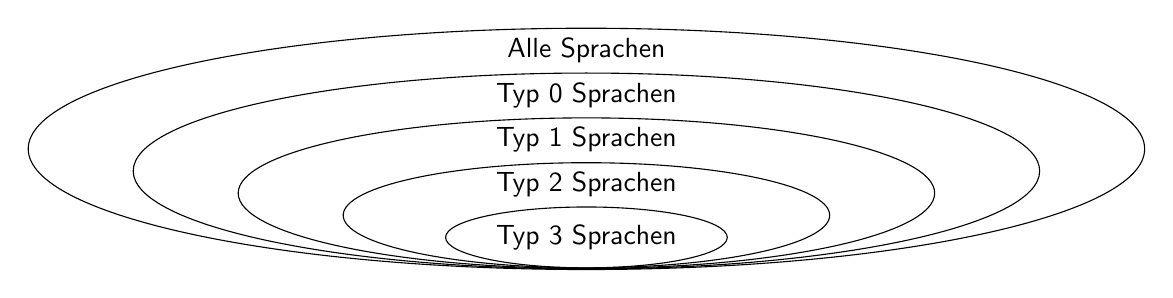
\begin{tikzpicture}[font=\sffamily,breathe dist/.initial=0.01ex]
\foreach \X [count=\Y,remember=\Y as \LastY] in
{Typ 3 Sprachen, Typ 2 Sprachen, Typ 1 Sprachen, Typ 0 Sprachen, Alle Sprachen}
  {\ifnum\Y=1
  \node[ellipse,draw,outer sep=0pt] (F-\Y) {\X};
  \else
  \node[anchor=south] (T-\Y) at (F-\LastY.north) {\X};
  \path let \p1=($([yshift=\pgfkeysvalueof{/tikz/breathe dist}]T-\Y.north)-(F-\LastY.south)$),
  \p2=($(F-1.east)-(F-1.west)$),\p3=($(F-1.north)-(F-1.south)$)
  in ($([yshift=\pgfkeysvalueof{/tikz/breathe dist}]T-\Y.north)!0.5!(F-\LastY.south)$)
  node[minimum height=\y1,minimum width={\y1*\x2/\y3},
  draw,ellipse,inner sep=0pt] (F-\Y){};
  \fi}
\end{tikzpicture}

%-----------------------------------------------------------------------
%
%-----------------------------------------------------------------------

\noindent
Die Sprache

\begin{itemize}
\item $L_3 = \{(ab)^n \, | \, n \in \mathbb{N}\}$
ist regulär (Typ 3 Sprache)

\item $L_2 = \{a^n b^n \, | \, n \in \mathbb{N}\}$
ist kontextfrei (Typ 2 Sprache), aber nicht regulär

\item $L_1 = \{a^n b^n c^n \, | \, n \in \mathbb{N}\}$
ist kontextsensitiv (Typ 1 Sprache), aber nicht kontextfrei

\item $L_0 = \{a^{(2^n)}\, | \, n \in \mathbb{N}\}$
ist eine Typ 0 Sprache\footcite[Seite 15]{theoinf:fs:1}
\end{itemize}

%-----------------------------------------------------------------------
%
%-----------------------------------------------------------------------

Ein Terminalsymbol (auch Terminalzeichen oder kurz Terminal genannt)
einer formalen Grammatik ist ein Symbol, das einzeln nicht weiter durch
eine Produktionsregel ersetzt werden kann.\footcite{wiki:terminal}

Eine Produktionsregel (auch Regel, Produktion oder Ersetzungsregel
genannt) ist in der Theorie formaler Grammatiken eine Regel, die angibt,
wie aus Wörtern durch eine Grammatik neue Wörter bzw. Symbolfolgen
produziert werden.\footcite{wiki:produktionsregel}

\section{Section}

\subsection{Grammatik reguläre Sprachen}

Sei $\Sigma$ ein Alphabet. Eine formale Sprache $L$ ist eine Teilmenge
aller Wörter über $\Sigma$:

\begin{displaymath}
L \subseteq \Sigma^*
\end{displaymath}

\bigskip

\noindent
Eine Grammatik ist ein 4-Tupel mit $G = (V, \Sigma, P, S)$ und besteht aus:

\begin{itemize}
\item Einer endlichen Menge $V$ von \memph{Variablen} (Nonterminale)

\item Dem endlichen \memph{Terminalalphabet} $\Sigma$ mit $\Sigma \cap V
= \emptyset$

\item Der endlichen Menge an \memph{Produktionen}

\item Und einer \memph{Startvariablen} $S$ mit $S \in V$
\end{itemize}

%-----------------------------------------------------------------------
%
%-----------------------------------------------------------------------

\section{Beispiel:}

$G = (V, \Sigma, P, S)$ mit

$V = \{Z, A\}$

$\Sigma = \{0, 1\}$

$P: Z \rightarrow 1a \,|\, 1$

$P: A \rightarrow 1A \,|\, 0A \,|\, 1$

Eine reguläre Sprache wird durch eine reguläre
Grammatik erzeugt, d.h. eine Grammatik mit
Produktionsregeln der Form:

$A \rightarrow \epsilon$ oder $A \rightarrow 1$ oder $A \rightarrow 0A$

linke Seite: ein Nonterminal rechte Seite: $\epsilon$ oder ein Terminal
oder ein Terminal gefolgt von einem Nonterminal

Man spricht hierbei auch von rechtslinearer Grammatik (es gibt auch
linkslineare Grammatiken)

$G = (\{Z, A\}, \{0, 1\}, P, Z)$

Syntaxbaum zu 100101
\begin{center}
\begin{tikzpicture}[level distance=0.7cm]
\Tree [.Z
  [.1 ] [.A
    [.0 ] [.A
      [.0 ] [.A
        [.1 ] [.A
          [.0 ] [.A
            [.1 ]
          ]
        ]
      ]
    ]
  ]
]
\end{tikzpicture}
\end{center}

%-----------------------------------------------------------------------
%
%-----------------------------------------------------------------------

\section{Deterministische endliche Automaten}

Ein deterministischer endlicher Automat (DEA; englisch deterministic
finite state machine oder deterministic finite automaton, DFA) ist ein
endlicher Automat, der unter Eingabe eines Zeichens seines
Eingabealphabetes (den möglichen Eingaben) von einem Zustand, in dem er
sich befindet, in einen eindeutig bestimmten Folgezustand wechselt.
\footcite{wiki:dea}

Automaten sind deterministisch, wenn es in jedem Zustand für jedes
Eingabesymbol höchstens einen (in einem vollständigen Automaten genau
einen) Folgezustand gibt.
\footcite[Seite 28]{vossen}

Ein DEA/DFA ist ein 5-Tupel ($Z, \Sigma, \sigma, E, z_0$) mit

\begin{description}
\item[$Z$:] Menge der Zustände (endlich)
\item[$\Sigma$:] Eingabealphabet mit (endlich)
\item[$\delta$:] $Z \times \Sigma \rightarrow Z$ Zustandsübergangsfunktion
\item[$E$:] Menge der Endzustände
\item[$z_0$:] Startzustand\footcite[Seite 26]{theoinf:fs:1}
\end{description}

%-----------------------------------------------------------------------
%
%-----------------------------------------------------------------------

\section{Minimierungsalgorithmus\footcite[Seite 47-57]{vossen}}

\footcite[Seite 51-62]{theoinf:fs:1}

https://studyflix.de/informatik/dea-minimieren-1212

%-----------------------------------------------------------------------
%
%-----------------------------------------------------------------------

\section{Nichtdeterministische endliche Automaten}

Ein nichtdeterministischer endlicher Automat (NEA; englisch
nondeterministic finite automaton, NFA) ist ein endlicher Automat, bei
dem es für den \memph{Zustandsübergang mehrere gleichwertige
Möglichkeiten} gibt. Im Unterschied zum deterministischen endlichen
Automaten sind die Möglichkeiten nicht eindeutig, dem Automaten ist also
nicht vorgegeben, welchen Übergang er zu wählen hat.\footcite{wiki:nea}

\begin{center}
\begin{tikzpicture}[->]
\node[state,initial] (p) {p};
\node[state,accepting,right=of p] (q) {q};

\path (p) edge[above] node{1} (q);

\path (p) edge[loop,above] node{0,1} (q);
\end{tikzpicture}
\end{center}

Nichtdeterministische endliche Automaten sind Automaten, in denen es zu
einem Zustand und einem Eingabesymbol mehrere Folgezustände geben kann.
\footcite[Seite 28]{vossen}

Ein NEA/NFA ist ein 5-Tupel ($Z, \Sigma, \sigma, E, z_0$) mit

\begin{description}
\item[$Z$:] Menge der Zustände (endlich)
\item[$\Sigma$:] Eingabealphabet mit (endlich)
\item[$\delta$:] $Z \times \Sigma \rightarrow 2^Z$ Zustandsübergangsfunktion
\item[$E$:] Menge der Endzustände
\item[$z_0$:] Startzustand\footcite[Seite 30]{theoinf:fs:1}
\end{description}

Potenzmenge

Beispiel: $Z = \{z_1, z_2\}$

$2^Z = \{\{\}, \{z_1 \}, \{z_2 \}, \{z_1 , z_2 \}\}$

\literatur

\end{document}
